\iffalse
%%%%%%%%%%%%%%%%%%%%%%%%%%%%%%%%%%%%%%%%%%%%%%%%%%%%%%%%%%%%
\chapter{FORMULACIJA PROSTORSKIH NOSILCEV PO GEOMETRIJSKO TO?NI 
		 TEORIJI Z NEZVEZNO KINEMATIKO}
%%%%%%%%%%%%%%%%%%%%%%%%%%%%%%%%%%%%%%%%%%%%%%%%%%%%%%%%%%%%
\thispagestyle{fancy}



%-----------------------------------------------------------
\section{Matemati?ni model nosilca}
\label{sec: Matematicni model}
%-----------------------------------------------------------

%
%\begin{figure}[ht]
%\begin{center}
%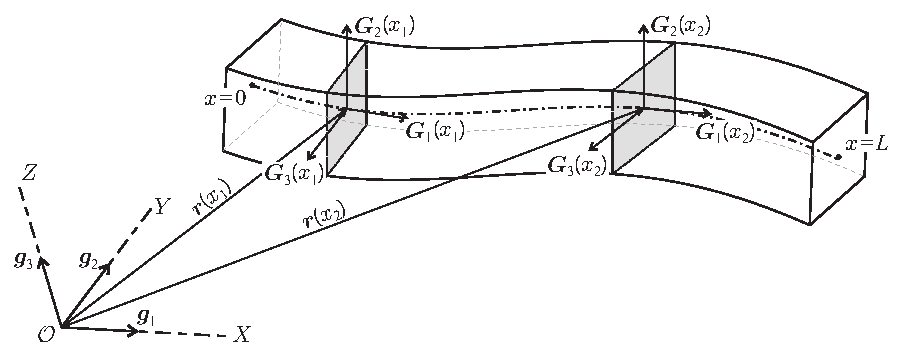
\includegraphics{FormulacijaZNezveznoKinematiko/slike/ModelNosilca}
%\bicaption[fig: Matematicni model nosilca]{}{
%Matemati�ni model nosilca.
%}{Figure}{
%Mathematical beam model.}
%\addfiguretolof{Mathematical beam model.}
%\end{center}
%\end{figure}
%




Vpeljemo dve bazi:
\begin{itemize}
\vspace*{-0.3cm}
\item[(i)] 	Prva je glede na prostor nepomi?na ortonormirana baza $\bs{g}$, 
			ki jo dolo?a trojica 
		    baznih vektorjev $\left\lbrace \bs{g}_1,\bs{g}_2,\bs{g}_3 \right\rbrace$,
		    pripetih v opazovali??e prostora. Nepomi?no bazo v literaturi imenujejo 
		    tudi prostorska ali globalna baza. Matrike, zapisane glede na prostorsko 
		    bazo, ozna?ujemo z indeksom $g$.
\vspace*{-0.7cm}		   
\item[(ii)] Druga je telesna baza 
			$\bs{G} = \left\lbrace \bs{G}_1(x),\bs{G}_2(x),\bs{G}_3(x) \right\rbrace$, 
			ortonormalna. V literaturi jo imenujejo tudi pomi?na ali lokalna baza. 
			Matrike, zapisane glede na telesno bazo, ozna?imo z indeksom $G$.
			Ker je njena pozicija v prostoru odvisna od trenutne rotacije pre?nega 
			prereza, je v splo?nem za vsak pre?ni prerez druga?na, torej odvisna od $x$. 
			Vektorji telesne baze so izbrani tako, da je vektor $\bs{G}_1$ pravokoten na 
			zavrteni pre?ni prerez, bazna vektorja $\bs{G}_2$ in $\bs{G}_3$ pa sta 
			usmerjena vzdol? glavnih vztrajnostnih osi prereza.
\end{itemize} 


\vspace*{-0.3cm}


%-----------------------------------------------------------
\section{Pomiki, rotacije in deformacije}
\label{sec: Pomiki, rotacije in deformacije}
%-----------------------------------------------------------
Geometrijsko to?na teorija reducira tenzorsko polje deformacij, ki je zvezno
porazdeljeno po volumnu nosilca, na dve deformacijski vektorski polji, vezani na 
materialne to?ke osi nosilca \cite{Reissner1981} - vektor translacijskih 
(vzdol?nih, pre?nih) deformacij in vektor rotacijskih deformacij  
(upogib, torzija), ki ju v matri?ni obliki ozna?imo z $\bs{\gamma}_G$ in $\bs{\kappa}_G$.
Njune komponente, $\gamma_1, \gamma_2, \gamma_3$  in 
$\kappa_1, \kappa_2, \kappa_3$, predstavljajo v trenutni telesni 
bazi pre?nega prereza $G$ osno in stri?ni deformaciji, 
torzijski zasuk in upogibni deformaciji - pseudoukrivljenosti. 
Iz principa virtualnega dela sledi, da krajevni vektor vzdol?ne osi nosilca  
in rotacijski vektor pre?nega prereza, ki ju v matri?ni obliki ozna?imo z $\bs{r}_{g}$ 
in $\bs{\vartheta}_{g}$, kakor tudi njuni variaciji 
$\delta\bs{r}_{g}$ in $\delta \bs{\vartheta}_{g}$, zado??ajo pogoju:
%
\begin{align}
\delta\bs{r}'_{g}\left( x \right) &= 
\bm{R}\left(x\right)\delta \bs{\gamma}_{G}\left( x \right) - 
\bs{r}'_{g}\left( x\right) \times
\delta \bs{\vartheta}_{g}\left( x \right) ,
\label{eq: sibka kinematicna enacba 1} \\
\delta\bs{\vartheta}'_{g}\left(x\right) &=
\bm{R}\left(x\right)
\delta\bs{\kappa}_{G} \left(x\right).
\label{eq: sibka kinematicna enacba 2}
\end{align}
%

Z integracijo ena?b \eqref{eq: sibka kinematicna enacba 1} in
\eqref{eq: sibka kinematicna enacba 2} glede na variacije dobimo zveze med krajevnim vektorjem in vektorji 
pomikov, rotacij in deformacij:
%
\begin{align}
\bs{r}'_{g}\left(x\right) & = \bm{R}\left(x\right)
\left( \bs{\gamma}_{G}\left(x\right) - \bs{\gamma}_{G}^{0} \left(x\right)\right),
\label{eq: kinematicna enacba 1} \\
\bs{\vartheta}'_{g}\left(x\right) &= \bm{T}^{-T} \left(x\right)
\left( \bs{\kappa}_{G}\left(x\right)-  \bs{\kappa}_{G}^{0} \left(x\right)\right).
\label{eq: kinematicna enacba 2}
\end{align}
%

\fi
